\documentclass[prd, showpacs,nofootinbib,amsmath,amssymb,12pt]{revtex4}
%\documentclass[aps,prd,showpacs,nofootinbib,preprintnumbers,twocolumn]{revtex4-1}
\usepackage{amsfonts, amssymb, amsmath, graphicx, comment, bm, slashed}
\usepackage[colorlinks]{hyperref}
\usepackage{dcolumn}
\usepackage{bm}
\usepackage[caption=false]{subfig}
\usepackage{multirow}
\usepackage{mathrsfs,cleveref}
\crefformat{equation}{Eq.~(#2#1#3)}
\crefformat{section}{Sec.~#2#1#3}



\begin{document}
\title{Magnetized color-flavor locked quark matter and its Bose-Einstein condensed phases in Nambu-Jona-Lasinio model with axial anomaly }
\author{xxx$^1$}
\author{xxx$^1$}
\author{xxx$^1$}
\author{xxx$^2$}
\affiliation{$^1$School of Physics, Nankai University,\\Tianjin  300071, China}
\affiliation{$^2$ Department of Physics, Shanghai Normal University,\\ Shanghai 200230, China}
% The "\note" macro will give a warning: "Ignoring empty anchor..."
% you can safely ignore it.

\date{\today}
\begin{abstract}
Previous studies show that there exist possible coexistence of diquark and chiral condensates and  critical phenomena in the moderate-density and zero-temperature quark matter,
as long as the QCD axial anomaly is considered.
In the three-flavor Nambu-Jona-Lasinio model with axial anomaly,
we take the influences of rotated electromagnetic field into account and explore the phase structure of  magnetized color-flavor-locked  matter.
Due to the coupling to rotated-charged quarks, the magnetic field is found to facilitate a specific diquark Bose-Einstein condensed phase that referred as $\text{BEC}_\text{I}$.
 With increasing magnetic field, the coexistence phase becomes superseded  by the newly defined $\text{BEC}_\text{I}$ phase gradually and the inverse magnetic catalysis happens for intermediate magnetic fields. For strong fields (say $eB>2.25\times10^{19}$G) , the $\text{BEC}_\text{I}$ existence makes the critical phenomena different from the zero field results   totally.
Also, it is observed that   $\text{BEC}_\text{I}$   occurs at relatively larger quark chemical potential and  relatively weak axial-anomaly coupling, which might be important for  the physics of magnetars.

\end{abstract}
\maketitle

\section{Introduction}
The phases of strongly interacting matter described by quantum chromodynamics (QCD) have attracted great interests for years.
The low-energy ground state of QCD is the hadron phase with condensation of quark-antiquark pairs,
namely the chiral condensate $\langle\bar{q}q\rangle$, and it undergoes transition to the quark-gluon plasma phase at high temperature.
At low temperature and high baryon number density,
the Bardeen-Cooper-Schrieffer (BCS) pairing mechanism among quarks has been proposed and the diquark condensate $\langle qq\rangle$ leads to various color-superconducting phases, see e.g. Refs.~\cite{alford2004dense,alford1998qcd} for reviews.
For three-flavor quark matter in the chiral limit, the color-superconducting phase corresponds to the color-flavor-locked (CFL) phase,
which suggests to be the ground state of QCD for very high densities~\cite{alford1998qcd}.
On account of these phases, many versions of QCD phase diagram were given schematically and,
in particular, several of QCD critical points were suggested theoretically in literatures.

Both the high-temperature critical phenomena and the low-temperature critical phenomena have been attracted attention recently~\cite{}.
The latter was firstly predicted by a Ginzburg-Landau (GL) analysis with the interplay between chiral and
diquark condensates induced by the QCD axial anomaly~\cite{yamamoto2007phase}.
It was further investigated in a phenomenological Nambu-Jona-Lasinio (NJL) model,
where the axial anomaly is taken into account by including the Kobayashi-Maskawa-'t Hooft six-quark effective interactions~\cite{abuki2010nambu}.
%incorporating the interplay between the chiral and diquark condensates induced by
Due to the chiral-diquark interplay,
not merely the coexistence (COE) of diquark and chiral condensates but also low-temperature critical phenomena are found to be different from the previous studies.
As detailed in Ref.\cite{abuki2010nambu},
the phenomenon takes place in the sense that a Bose-Einstein condensation (BEC) of diquark molecules emerges firstly
and then a crossover between the BEC phase and the BCS-type CFL phase is realized.

Critical phenomena in the low-temperature could not be addressed with the first-principle lattice QCD simulations.
Its existence is difficult to be observed in experimental heavy ion programs directly.
The NJL calculations of this critical point are highly model dependent.
Also, whether the low-temperature critical phenomena exist or not was found to be sensitive to a specific chiral-diquark coupling crucially\cite{}.
Even for the appropriate model parameters, the given COE region is rather narrow and the obtained critical point is located at the intermediate density\cite{abuki2010nambu}.
More importantly, the locations of such critical phenomena and their existences are still unclear in reality environment.
For instance, if bare quark mass is included, $BEC$ would exclude from the phase diagram and the $2SC_{BEC}$ emerge Ref.~\cite{basler2010role}.
Also, the effect of confinement was found to relate with Polyakov loop Ref.~\cite{Powell2011Axial}, which indicate the existence of $BEC$.
In the Ref.[], the local charge-neutrality are not considered.
Those problem need further discussion.

On the other hand, the effect of magnetic field in the color superconductor (CSC) matter was studied by many authors~\cite{ferrer2006color,ferrer2007magnetic,ferrer2005magnetic,fukushima2008color,fayazbakhsh2010color,fayazbakhsh2011phase,mandal2013neutrality,mandal2016effect,mandal2017effect}.
It is believed that there exist strong magnetic fields in the astrophysical "Laboratories".
Magnetic fields of the order of $B \sim 10^{14}$ - $10^{15}\text{G}$ can be observed on the surface of Magnetars.
In the interior of compact stars, the strengths can reach $B \sim 10^{18}\text{G}$ and a theoretical upper limit may be up to $B \sim 10^{20}\text{G}$~\cite{dong2001,lai1991cold}.
Some of recent works were devoted to magnetic effect on the CFL color-superconducting phase.
In this case, the rotated electric charge $\widetilde{Q}$ defined in the color-flavor space
and the rotated electromagnetic mechanism play the key roles since the unbroken symmetry is $U(1)_{\widetilde{Q}}$~\cite{alford1998qcd,alford2000mg}.
Once an unscreened magnetic field $B$ are turned on, considerable changes are predicted in CFL.
According to the rotated-charges of quark species, in particular, different magnetic responses lead to the splitting of diquark condensate,
and the correspond CSC gaps ~\cite{ferrer2005magnetic,fukushima2008color,ferrer2006color,ferrer2007magnetic}.
%In Ref.\cite{}, an inverse magnetic catalysis for the emergence of diquark BEC phase was found under certain circumstance of magnetic field and the influence on such a BEC-BCS crossover was investigated.
%It is worth to note that the phenomenon around this BEC-BCS crossover is not the above-mentioned critical phenomenon that predicted in three flavor and color QCD system \cite{}.
%For the latter, to the best of our knowledge, the magnetic effect have not yet been elucidated until now.
Noted that the only place CSC might be observed is the interior region of compact stars, many studies pay attention to the magnetic effect on the CSC  phase.
For example, the gap splitting are considered when the magnetic field is introduced to BCS phase of CSC.
It is important and crucial to investigate the relationship between COE, BEC and critical phenomena.
Since there exist both chiral-condensate and diquark-condensate in COE, the magnetic field influence in expected to be manifold and complicated.
In NJL-model with axial anomaly in the presence of magnetic effect have not yet been included.
Exploring this effects is the main purpose of present paper.
%This topic would lay the foundation for the well-resourced phase diagram and possible applications for the physics of magnetars and it is one of the important problems in the context of strongly interacting matter under magnetic fields.

The paper is organized as follow.
In section 2, we study COE phase and critical phenomena in the presence of $B\neq0$, and expand NJL-model with axial anomaly.
%incorporate an applied field $B$ into the NJL model with axial anomaly to study how the chiral-diquark interplay and low-temperature critical point be modified by the presence of magnetic fields.
%Due to the rotated electromagnetic mechanism, there exist the splitting of diquark condensate, namely,
%rotated-charged($\widetilde{Q}$)  and rotated-neutral diquark gaps or channels.
%As magnetic field is introduced, the critical phenomenon changes comparing with zero field resulting.
The diquark condensates are found to split into the rotated-charged relevant one $s_B$ and the irrelevant one $s$,
which shares one similarity with the gap splitting in the ``pure" CFL phase without chiral condensate.
As the consequence, the mean-field thermodynamic potential behaves as the function of three condensates $s_B$,
$s$ and $\chi$ at the given temperature and quark chemical potential.
By employing the extended formalism, our attention is first paid to the ${\widetilde{Q}}$-relevant channel of diquark condensate.
We find that its associated BEC critical point are facilitated significantly by the presence of magnetic fields.
%Then we study how the axial-anomaly induced interplay between chiral and diquark condensates be modified under magnetic fields.
%We find that the interplay itself is facilitated also, which supports the existence of low-temperature critical point totally.
%Our results suggest that this results are caused by the competition of inverse IMC in diquark condensate and MC effect in chiral condensate.
In section 3, we give our numerical result in the two different magnetic field value to illustrate the phenomena,
compared with the zero-field case, in the presence of the magnetic field.
In section 4, we mainly to discuss the different effect happened in the both sides of the threshold value.

\section{The NJL model of magnetized CFL matter with axial anomaly}

The formalism of NJL-model with axial anomaly in zero magnetic field is firstly reviewed \cite{abuki2010nambu}.
Then, we expand this formalism with non-vanishing magnetic fields.
Finally, we will give the regularization scheme and model parameter.

\subsection{Model formalism in the absence of magnetic  field}
\label{sec:2a}
In general, the NJL-type Lagrangian\cite{abuki2010nambu} reads
\begin{equation}
	\mathcal{L} = \bar{q} (i\gamma^\mu \partial_\mu + \gamma_0\mu +m_q) q +
	\mathcal{L}^{(4)}+ \mathcal{L}^{(6)},
	\label{eq:lag}
\end{equation}
where $\mu$ is the quark chemical potential, and $m_q$ is the current quark mass.
The four-quark interaction $\mathcal{L}^{(4)}$ are consists of $\mathcal{L}^{(4)}_\chi$ and $\mathcal{L}^{(4)}_s$, 
which refer to the $qq$ and $q\bar{q}$ channel respectively.
The six-quark interaction, causing by the axial anomaly, 
consists of two parts $\mathcal{L}^{(6)}=\mathcal{L}^{(6)}_{\chi}+\mathcal{L}^{(6)}_{\chi s}$. 
For 3-color and 3-flavor quark matter, the chiral condensates are defined as 
\begin{equation}
\chi\delta_{ij}= \langle\bar{q}_i q_j\rangle,\quad
\end{equation}
where the (i,j,k) are flavor indices for (s,d,u).
The diquark condensates are defined as 
\begin{equation}
s\delta_{AA'}=\langle q^TC\gamma_5\tau_A\lambda_{A'} q\rangle,
\end{equation}
where $\tau_A$ and $\lambda_{A'}$ is Gell-Mann matrices in color and flavor space respectively.
The flavor and color structure of the diquark interaction is generated by the anti-symmetric matrices($A,A'=2,5,7$), 
thus the diquark condensate classified as $s_{22}, s_{55}, s_{77}$.
In the absence of magnetic field, quark color superconductor phase correspond to the $CFL$ matter, 
where the unique diquark condensate $s=s_{22}=s_{55}=s_{77}$.

In the mean-field approximation, the interaction terms in Eq.(\ref{eq:lag}) can be written as\cite{abuki2010nambu},  
\begin{equation}
\mathcal{L}^{(4)}_{\chi}=4G\chi\bar{q}q-6G\chi^2.
\end{equation}	
\begin{equation}
\mathcal{L}^{(4)}_{s}=H[s^*(q^TC\gamma_5\tau_A\lambda_Aq)+h.c.]-3H|s|^2.
\end{equation}
\begin{equation}
\mathcal{L}^{\left(6\right)}_{\chi}=-2K\chi^2\bar{q}q+4K\chi^3.
\end{equation}
\begin{equation}
\mathcal{L}^{\left(6\right)}_{\chi s}=-\frac{K'}{4}|s|^2\bar{q}q-\frac{K'}{4}\chi[s^*(q^TC\gamma_5\tau_A\lambda_Aq)+h.c.]+\frac{3K'}{2}|s|^2\chi.
\end{equation}
In the four-quark interaction, the couplings for $qq$-channel and $q\bar{q}$-channel are $G$ and $H$ respectively.
$\mathcal{L}^{\left(6\right)}_{\chi}$ is the standard Kobayashi-Maskawa-'t Hooft interaction which couples the chiral condensate only.
And the interaction coupling is written as $K$.
For the six-point term $\mathcal{L}^{\left(6\right)}_{\chi d}$ with coupling $K'$, it corresponds to the interplay between chiral and diquark condensates.
Based on equations above, 
all the $q\bar{q}$-channel interaction terms can be attributed as  the constituent quark mass (the dynamic Dirac mass)
\begin{equation}
M = -4(G-\frac{1}{8}K\chi)\chi + \frac{1}{4}K's^2.
\label{Dmass}
\end{equation}
We will ignore the current quark mass $m_q$ all through this work.
The constituent mass is not only made up by four-quark interaction with $G$,
but also related to the Kobayashi-Maskawa-'t Hooft interaction of six-quark interaction $K$ and the chiral-diquark interplay $K'$, 
which would introduce the axial anomaly.

Similarly, the $qq$-channel  interaction can be given as the color-superconductor gap (the dynamic Majorana mass)
\begin{equation}
\Delta=-2Hs+\frac{1}{2}K'\chi s.
\end{equation}
Besides the four-quark interaction with coupling $H$, the chiral-diquark interaction with $K'$ also plays an important role.
For $qq$-channel, we will define the effective coupling parameter as
\begin{equation}
\label{eq:effectivecoupling}
H'=H - \frac{1}{4}K'\chi,
\end{equation}
so that the diquark gap is given as $\Delta=-2H's$. 
Therefore, the additional chiral-diquark interplay enhance the diquark coupling.
This is the essential reason that the axial anomaly raise the COE of chiral and diquark condensates and thus diquark BEC phase occur
We will investigate this effective coupling with magnetic field in the later section.

In the absence of magnetic field, the thermodynamic potential is usually written as 
\begin{equation}
\Omega=\Omega_q+U(\chi,s).
\end{equation}
By using the Nambu-Gor'kov formalism in zero temperature, 
the one-loop contribution given as\cite{abuki2010nambu},
\begin{equation}
\Omega_q=-8\sum_{\pm}\int^{\Lambda}_0\frac{d^3p}{(2\pi)^3}|\epsilon^8|
-\sum_{\pm}\int^{\Lambda}_0\frac{d^3p}{(2\pi)^3}|\epsilon^1|,
\label{oneloopinzero}
\end{equation}
(is this int form 0 to Lambda) where the sum indices of $\pm$ represent the quasiparticle and anti-quasiparticle excitations respectively.  
And the $\Lambda$ is the re-normalization factor for our model parameter.
The dispersion relation in singlet and octet representations reads
\begin{equation}
\epsilon^1=\sqrt{(E\pm\mu)^2+(2\Delta)^2},\quad
\epsilon^8=\sqrt{(E\pm\mu)^2+\Delta^2},
\label{despersionzerofield}
\end{equation}
with the single-particle energy $E=\sqrt{p^2+M^2}$ .
Besides, the interaction potential $U$ reads
\begin{equation}
U(\chi,s) = 6G\chi^2 - 4K\chi^3 + 3(H-\frac{K'}{2}\chi)s^2.
\label{potentialterm}
\end{equation}

\subsection{Formalism in the presence of magnetic field}
Now we turn to the formalism of the magnetized CFL matter. 
In a NJL model (without axial anomaly), 
its BCS phase has been intensively studied in the Refs.\cite{ferrer2005magnetic,Fukushima2008Color,Ferrer2006Color}.
The most important physics is the rotated-electromagnetic mechanism.\cite{alford1998qcd},
namely the unbroken symmetry is described by the subgroup $U(1)_{\widetilde{Q}}$,
with $\widetilde{Q}=Q\times\bm{1}+\bm{1}\times T_8/\sqrt{3}$, 
where $Q=\text{diag}(-\frac{1}{3},-\frac{1}{3},\frac{2}{3})$ for $(s,d,u)$ and $T_8=\text{diag}(-\frac{1}{\sqrt{3}},-\frac{1}{\sqrt{3}},\frac{2}{\sqrt{3}})$ for $(b,g,r)$.
And the rotated magnetic field becomes linear combination of an usual photon and the eighth gluon fields.
Consequently, the unique diquark condensate $s$ defined in section becomes two condensates $s\equiv s_{22}$ and $s_B\equiv s_{55}=s_{77}$
in CFL matter split into two the diquark condensates $s=s_{22}$ and $s_B=s_{55}=s_{77}$.
According to the $\widetilde{Q}$ properties of quarks, there actually exist the threes types of pairing patterns:
the neutral, charged and mixed pairings as summarized in Table \ref{tab:1}.\cite{ferrer2005magnetic}.

\begin{table}[ht]
\label{tab:1}
  \caption{classification of pairings, gaps and dispersion relations}
  \centering
   \begin{tabular}{c|c|c|c|c}
    \hline\hline
    Paring  type           & neutral               & mixed                         & \multicolumn{2}{c}{charged}\\
    \hline
    Quark                  & bd\quad gs            & ru\quad gd\quad bs            & rs\quad bu  & gu\quad rd\\
    \hline
    $\widetilde{Q}$        & 0\quad 0              & 0\quad 0\quad 0               & +1\quad -1  & -1\quad +1\\
    \hline
    Diquark condensate     & $s$                   & $s$\quad $s_B$                & \multicolumn{2}{c}{$s_B$}\\
    \hline
    Gap                    & $\Delta$              & $\Delta_1,\Delta_2$           & \multicolumn{2}{c}{$\Delta_B$}\\
    \hline
    Dispersion relation    & $\epsilon^n$          & $\epsilon^m_1,\epsilon^m_2$   & \multicolumn{2}{c}{$\epsilon^c$}\\
    \hline\hline
   \end{tabular}
\end{table}

For the neutral type ( $bd-gs$ pairing), only the diquark condensate $s$ is involved and the color superconductor gap is determined by it.
In the NJL-model with axial anomaly, the gap reads
\begin{equation}
\Delta=-2H's.
\end{equation}
Correspondingly, the dispersion relation  has the form like 
\begin{equation}
\label{eq:disperzero}
\epsilon^n=\sqrt{(E\pm\mu)^2+\Delta^2},
\end{equation}
for the quark and anti-quark excitations respectively.
In Eq.\eqref{eq:disperzero}, the single particle energy is still $E=\sqrt{p^2+M^2}$ , although the quark mass in Eq.\ref{Dmass} needs to be modified(see below).
The neutral pairing contributes one-loop thermodynamic potential
\begin{equation}
\Omega^n_q=-6\sum_{\pm}\int h_{\Lambda}\frac{d^3p}{(2\pi)^3} |\epsilon^n|,
\label{omegaq}
\end{equation}
where the smooth regulator function $h_\Lambda$ has replaced the cut-off regulator scheme in Eq.\ref{oneloopinzero}.

For the charged type, the paired quarks carry the non-zero rotated charges (the $rs-bu$ and/or $gu-rd$ pairing, see Table \ref{tab:1}).
The gap is determined by the diquark condensate $s_B$,
\begin{equation}
\Delta_B=-2H's_B.
\end{equation}
In this case, the single -particle energy spectrum becomes Landau-levels
\begin{equation}
\label{eq:energyb}
E_B=\sqrt{p^2_3+M^2 + 2neB},
\end{equation}
where $p_3$ is the third component of momentum space, and $n$ is Landau level index($n=0,1,2,...$).
The dispersion relation for quasiparticle and anti-quasiparticle read:
\begin{equation}
    \epsilon^c=\sqrt{(E_B\pm\mu)^2+\Delta_B^2},
\end{equation}
where the gap $\Delta_B=-2H' s_B$.
By using the substitution:
\begin{equation}
2\int\frac{d^3p}{(2\pi)^3}\rightarrow\frac{eB}{8\pi^2}\sum^{\infty}_n(2-\delta_{n0})\int^{+\infty}_{-\infty} dp_3,
\label{eq:momentumsub}
\end{equation}
one can derive the themody-potential contribution from charged quarks in the present of magnetic fields.
For given cut-off parameter $\Lambda$, we introduce the number of completely occupied Landau levels $n_{max}$,
\begin{equation}\label{eq:nmax}
  n_{max}= \text{Int}[\frac{\Lambda^2}{2eB}],
\end{equation}
and obtain the one-loop thermodynamic potential 
\begin{equation}
\Omega^c_q=-8\sum_{\pm}\frac{eB}{8\pi^2}\sum_{n=0}^{n_{max}} (2 -\delta_{n0}) \int h^n_{\Lambda,B} dp_3|\epsilon^c|, 
\end{equation}
where $h^n_{\Lambda,B}$ is smooth regularization function for the charged pairing. Together with $h_\Lambda$ will be discussed in the following section.

For the mixed type(i.e. $ru-gd-bs$ pairing),  both $s$ and $s_B$ play their roles.
As detailed in Ref.\cite{Ferrer2006Color,noronha2007color},
the color-superconductor gaps behave as the combination of $\Delta$ and $\Delta_B$,
\begin{equation}
\Delta_{1}=\frac{1}{2}(\sqrt{\Delta^2 + 8\Delta_B^2} + \Delta),\quad
\Delta_{2}=\frac{1}{2}(\sqrt{\Delta^2 + 8\Delta_B^2} - \Delta).
\end{equation}
And the dispersion relation given as
\begin{equation}
\epsilon^m_1=\sqrt{(E\pm\mu)^2+\Delta_1},\quad \epsilon^m_2=\sqrt{(E\pm\mu)^2+\Delta_2}
\end{equation}
Since only the neutral quarks take a part in the mixed pairing,
the thermodynamic potential contribution reads \cite{noronha2007color}
\begin{equation}
\Omega^m_q=-2\sum_{\pm}\int h_{\Lambda}\frac{d^3p}{(2\pi)^3}  \epsilon^m_1 -2\sum_{\pm}\int h_{\Lambda}\frac{d^3p}{(2\pi)^3}  \epsilon^m_2.
\end{equation}

Now we turn to investigate the constituent  mass in the magnetized CFL matter.
Recalling that it stems the interacting terms in the $\bar{q}q$ channel, which is irrelevant to
$qq$ channel. $M$ has the similar form as Eq.(\ref{Dmass}), as long as the  splitting of
diquark condensate is taken into account.
While the first term in R.H.S. of  Eq.(\ref{Dmass}) 
holds unchanged, the splitting  changes the second term of Eq.(\ref{Dmass})
through the chiral-diquark coupling $K'$.
Due to  a simple relation $s^2_{22}+s^2_{55}+s^2_{77} = s^2 + 2s_B^2$ , 
the zero-field result $s^2$ should be replaced  $\frac{1}{3}s^2+\frac{2}{3}s^2_{B}$
in the presence of magnetic field.
Thus Eq.(\ref{Dmass}) in the zero-field result is rewritten as
\begin{equation}
M=-4(G-\frac{1}{8}K\chi)\chi+\frac{1}{12}K's^2+\frac{1}{6}K's^2_B,
\end{equation}
Following the same procedure, the interaction potential term Eq.\ref{potentialterm} is given by
\begin{equation}
U(\chi,s,s_B)=6G\chi^2-4K\chi^3+(H-\frac{K'}{2}\chi)(s^2+2s^2_B).
\end{equation}
Instead of Eq., the  total thermodynamic potential is the function of 
\begin{equation}

\Omega(\chi,s,s_B)=\Omega^n_q+\Omega^m_q+\Omega^c_q+U.
\label{finaleq}
\end{equation}
In Eq.~\eqref{finaleq}, the contribution from electromagnetic field (say, $\frac{1}{2}B^2$) in this equation has been dropped out, since the magnetic filed penetrate the CFL quark matter freely \cite{ferrer2005magnetic,  Ferrer2006Color,  ferrer2007magnetic}. 
Our calculations mainly based on the gap equations, which global minimizing the thermodynamic potential in order parameter space,
\begin{equation}
\frac{\partial\Omega}{\partial s} =0,\quad 
\frac{\partial\Omega}{\partial s_B} =0,\quad 
\frac{\partial\Omega}{\partial \chi} =0.
\end{equation}

\subsection{Model parameters and Regularization scheme}
\label{sec:2c}
In order to eliminate the unphysical oscillation, 
we have consider smooth regularization function $h_{\Gamma}$ for neutral part and $h^n_{\Gamma, B}$ for magnetic case.
For better illustration of our result, 
we choose the function so-call "Lorenzian type" \cite{Frasca2011Magnetic},
\begin{equation}\label{eq:regulator}
  h_{\Lambda} = [1+(\frac{p}{\Lambda})^5]^{-1}, \quad  h^n_{\Lambda,B}=[1+(\frac{\sqrt{p_3^2 + 2neB}}{\Lambda})^5]^{-1}.
\end{equation}
The numerical calculations in constituent quark mass show that, for our model, $n=5$ in Eq.\eqref{eq:regulator} 
has lesser oscillation behavior than the normal type like $n=15$ case and exponential cutoff.

To this end, it should be stressed that van Alphen-de Haas(vA-dH) oscillation happened in gaps (including $\delta$, $\delta_B$ and $M$) still exist.
Recent study suggested a new regulator scheme named "Magnetic Field Independent Regularization"\cite{allen2015magnetized}.
In Ref.\cite{allen2015magnetized}, the NJL-type model is investigated by using this regularization procedure in which the contributions that are explicitly dependent on the magnetic field turn out to be finite and do not required to be regularized. 

As for the model parameters, in order to perform the momentum integral numerically, we have to fix the cutoff $\Lambda$, 
four-fermion $(G,H)$ and six-fermion coupling constants $(K, K')$.
The momentum cutoff $\Lambda$ and the chiral coupling constant $G$ is fixed by fitting the pion prosperities in vacuum, e.g.,
the pion mass $m_\pi = 134 MeV$ and the constituent quark $M = 340 MeV$.
Besides, the diquark coupling constant $H$ is fixed by fitting the scalar diquark mass.
And the six-fermion coupling constants $(K, K')$ is maintained to make the second-order transition appear.
In the present work, we adopt the parameters setting in Ref.\cite{abuki2010nambu} (the first line of Table I in Ref.\cite{abuki2010nambu}).

\section{Numerical calculations}
\subsection{COE phase region in the presence of magnetic fields}
\label{sec:3a}
Firstly, we focus on the case of intermediate-magnetic fields. 
We plot  $\Delta$, $\Delta_{B}$ and $M$ as functions of chemical potential $\mu$ in Fig.\ref{f2}, 
and consider the magnetic field strength $eB=4.6m^2_\pi \simeq 1.40\times10^{19}$G.
Before introducing the phase diagram, two special phase should be defined.
Associated with the diquark gaps $\Delta$ and $\Delta_B$, 
we refer the diquark Bose-Einstein-condensate phase with $s=0, s_B\neq 0, \chi \neq 0$ as $BEC_I$ phase.
The BEC phase is defined as $s \neq 0, s_B \neq 0, \chi \neq 0$.

\begin{figure}[ht]
	\centering
	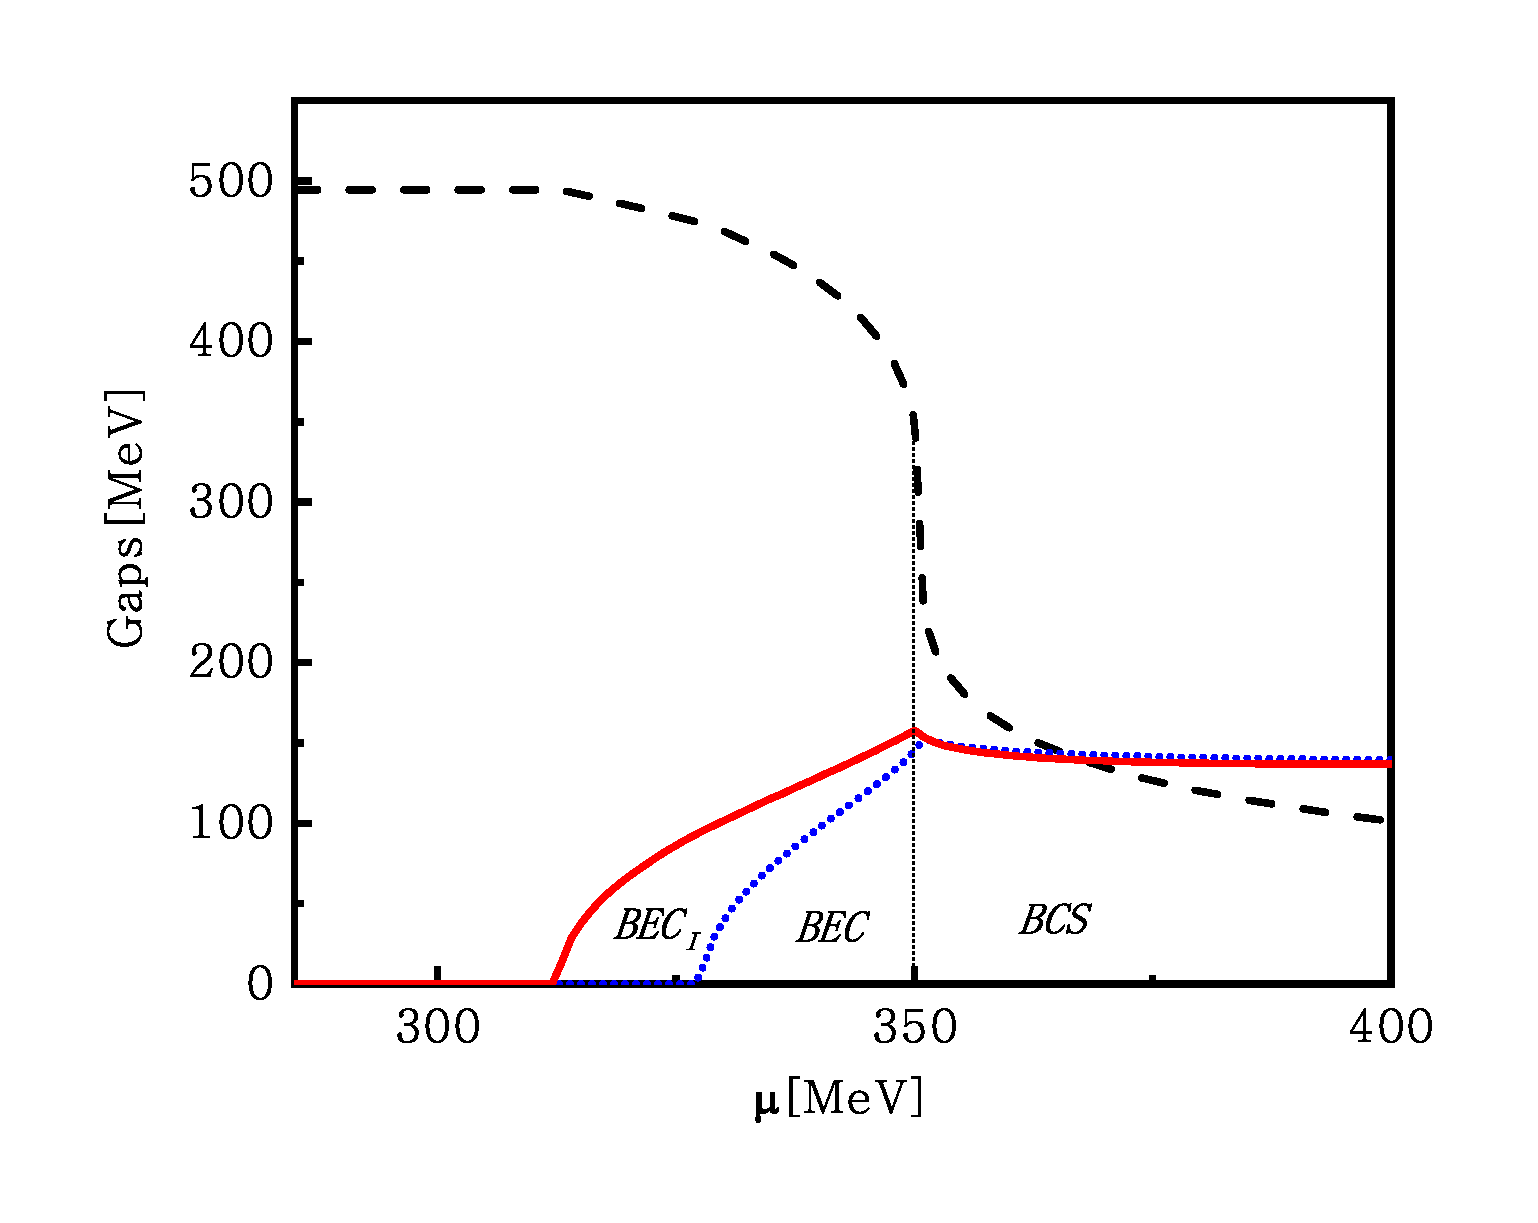
\includegraphics[scale=0.3]{1.eps}
	\caption{The constituent quark mass $M$(dashed-line), and color-superconductor gaps for diquark condensate $\delta$(blue dotted line) and $\delta_B$(red solid line) as functions of $\mu$ under the magnetic field value $eB/m^2_\pi=4.6$.}
	\label{f2}
\end{figure}

As shown in Fig.\ref{f2}, the $BEC_I$ phase occurs firstly before the $BEC$ phase.
Moreover, the $BEC_I$ phase would gradually occupies the COE region with the increasing magnetic field, 
and the BEC phase would be suppressed.
Another important physics is BEC-BCS crossover form $BEC$ phase to $BCS$ phase at $\mu_X = 350 MeV$,  
which determined by the quasi-particle dispersion relations.
For $\mu<M$, the minimum of the dispersion relations locates at $p=0$, the structure characteristic of the BCS phase.
For $\mu > M$, the minimum is shifted to $p = \sqrt{\mu^2-M^2}$ and quasi-particle gap is given by $\Delta$.
This corresponds to the fermionic spectrum in the BCS state.
Therefore the BEC-BCS crossover  is characterized by the condition $\mu =M$, and we define this reference chemical potential as $\mu_X$.

Compared to zero-field case, 
the Bose-Einstein-condensed phase also occurrence before BEC-BCS crossover.
The difference is COE region have two phase $BEC_I$ and $BEC$, which occur early then crossover.
In chemical potential section $313$ to $350$, the COE region still have the critical phenomena.

Secondly, when the magnetic field value greater a threshold value $eB_{th}$, 
numerical calculations show that the phase would be totally different from Fig.\ref{f2}.
In Fig.\ref{f3}, we give the result of $eB = 9.2m^2_\pi \simeq 2.80\times10^{19}$G .
The COE phase region is completely occupied by the $BEC_I$ phase and the $BEC$ phase disappeared. 
Different form the result of intermediate-field (includes zero-field),
constituent quark mass $M$ dramatically decreases and the value of $\delta$ jump from zero.
It implies that the second order transition in Fig.\ref{f2} turns to 1st order transition.
In other words, the phase at $\mu_X=338MeV$ are no longer critical phenomena.

\begin{figure}[ht]
	\centering
	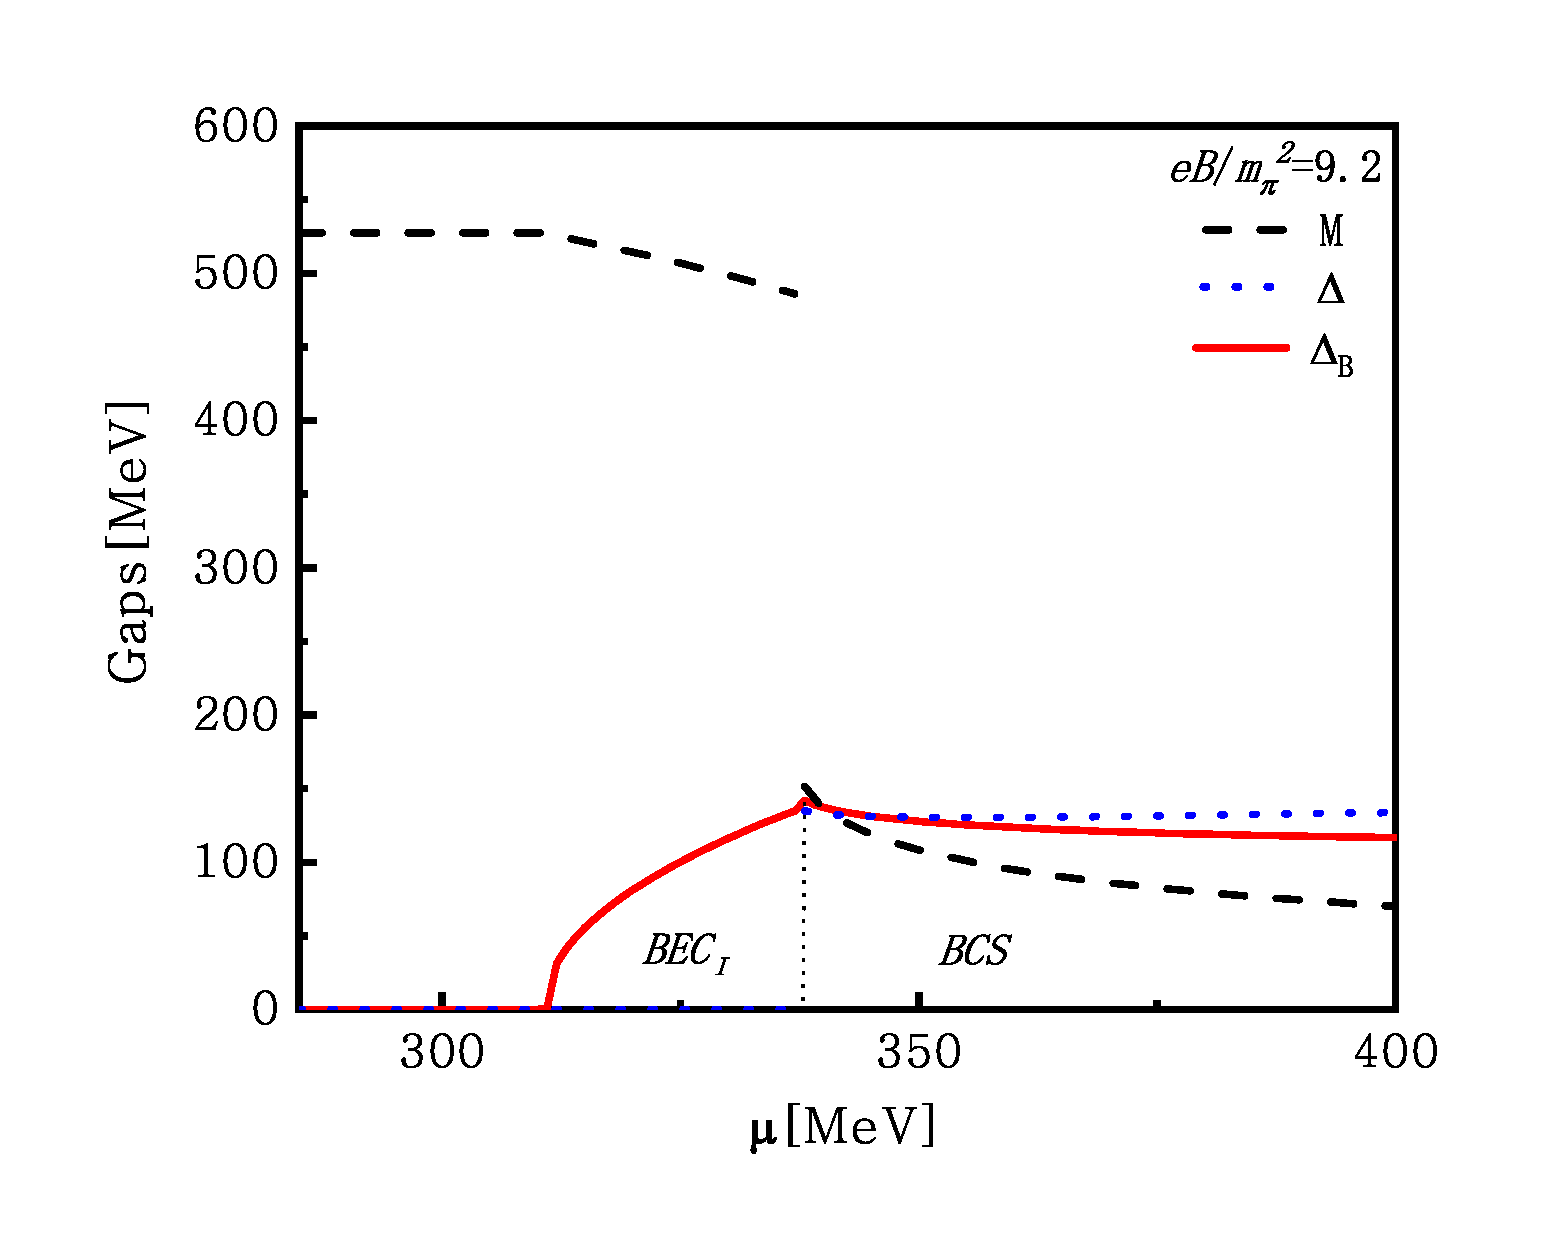
\includegraphics[scale=0.3]{2.eps}
	\caption{Similar as Fig.\ref{f2}, but for magnetic filed $eB/m^2_\pi$ equals to $9.2$.}
	\label{f3}
\end{figure}

Thus, introducing strong magnetic field have changed the COE phase and the zero-temperature critical phenomena caused by the axial anomaly previously predicted in Ref.\cite{abuki2010nambu}.
Physically, this reason can conclude to the CFL symmetry violation.
For intermediate-field, the violation of CFL phase cause the spliting of COE region to $BEC_I$ and $BEC$ phase.
Meanwhile, mechanism result to critical phenomena have no difference with zero-field case.
For strong-field, the symmetry is totally broken. 
In this case, COE region is occupied by $BEC_I$ and BEC-BCS no longer appear.

\subsection{Critical chemical potential for different BEC occurrences}
In order to further understand the phase structure obtained in Sec.\ref{sec:3a}, our attention is paid to the criteria  of diquark Bose-Einstein condensed phases.
As the second-order transition, the occurrence of a designated BEC phase can be determined by the Thouless criterion\cite{Nishida2005BCS}, i.e.,
%Now we try to explain the critical phenomena by investigating the criterion condition for the occurrence of  BEC phases.
%Considering the second order fluctuations around diquark gaps determined the mean-field approximation,
%the BEC criterion condition have been derived as \cite{Nishida2005BCS}
\begin{equation}\label{eq:omegasecond}
 \frac{1}{H'}= Q(\vec{q} =0, \omega =0),
\end{equation}
where $H'$ is effective diquark coupling in Eq.~\eqref{eq:effectivecoupling} and $Q(\vec{q},\omega)$ is diquark polarization function and can be derived from the usual
quark propagator at one-loop level\cite{}.

%where $Q_i$ is the  one-loop quark-quark polarization function and $i$ represents the diquark pairing .

% with the  quark fermion propagator $G_0(\vec{p}, 0) = [\slashed{p}+\mu\gamma_0 - M]^{-1} $.
%Since the occurence of BEC  can be treated as  a second-order phase transition for the corresponding diquark gaps,
%the second-order coefficient being zero determines the critical chemical potential for the BEC phase, i.e.,
%\begin{equation}
%\label{eq:bdiquark}
%	\alpha_2 \sim \frac{1}{H'} - Q_A(\vec{q} = \vec{0},\omega =0) =0.
%\end{equation}
%%This is just the Thouless criterion\cite{Nishida2005BCS} that widely used in condensed matter physics.
%The one-loop quark-quark polarization function  $Q_A$ in Eq.~\eqref{eq:omegasecond} can be archived by
%\begin{equation}
%\label{eq:qqpol}
%Q_A(\vec{q})
%= 2i\int \frac{d^4\vec{p}}{(2\pi)^4}
%\times \text{Tr}[i\gamma_5G_0(\vec{q}-\vec{p})i\gamma_5 C G_0(\vec{p})],
%\end{equation}
%with the  quark fermion propagator $G_0(\vec{p}, 0) = [\slashed{p}+\mu\gamma_0 - M]^{-1} $.



In the absence of magnetic field, the 
polarization function is easily obtained and the criterion of BEC occurrence reads
\cite{abuki2010nambu},
\begin{equation}\label{eq:criticalfor0}
  \frac{1}{4H'} =  4\sum_{\pm}\int \frac{d^3p}{(2\pi)^3} \frac{1-2f(E\pm \mu)}{2(E \pm \mu)}dp ,
\end{equation}
where $f(\epsilon) =1/(e^{\epsilon/T} +1)$ is the Fermi distribution function.
Under zero-temperature condition,  Eq.~\eqref{eq:criticalfor0} has  the form
\begin{equation}
\label{eq:criticalfor1}
\frac{1}{H'} = \frac{8}{ \pi^2} \int_0^\Lambda\frac{ E p^2}{E^2 - \mu^2} dp,
\end{equation}
where $E$ is the single particle energy and the  hard cut off regulator scheme is included. 

Once the magnetic field is introduced,   the splitting of diquark condensate leads to  Bose Einstein Condensed structure more complicated.
Different from the BEC phase with non-vanishing $s$ and $s_B$, here we has defined the condensed phase with  $s\neq 0$, $s_B=0$ as
 $\text{BEC}_\text{I}$ in Sec.\ref{sec:3a} . Besides,  the phase with $s\neq 0$, $s_B=0$ and $\chi  \neq 0$
 is theoretically possible,  which is referred as  $\text{BEC}_\text{II}$.
Let's firstly consider  the criterion of  $\text{BEC}_\text{II}$  occurrence.
%the diquark condensate in the order parameter is $s$.
The paired quarks involved in   $\text{BEC}_\text{II}$ (the diquark condensate  $s$)  are totally neutral.
So that, there is no the direct coupling to magnetic field. Similar to Eq.~\eqref{eq:criticalfor1}, 
the $\text{BEC}_\text{II}$ occurrence can be given as
\begin{equation}
\label{eq:criticalforn}
\frac{1}{H'} =\frac{8}{ \pi^2} \int h_\Lambda  \frac{ E p^2}{E^2 - \mu^2} dp,
\end{equation}
%Compared with Eq.~\eqref{eq:criticalfor0}, the criterion equation of $\text{BEC}_\text{II}$ is formally equivalent with that obtained in the case of $B = 0$,
%excepted that we have introduced 
where the smooth regulator function $h_\Lambda$ is introduced in the presence of magnetic field.

For the $\text{BEC}_\text{I}$ occurrence, the order parameter of diquark condensate  is $s_B$.
As shown in Table.\ref{tab:1}, there exist rotated-charged pairing (ud and us pairing) and neutral pairing (the mixed pairing).
Besides the single  particle energy $E$ , 
Eq.~\eqref{eq:energyb} for the rotated-charged quarks needs to be considered.
%$G_0(\vec{p},0) = [\slashed{p}_{\pm}+\mu\gamma_0 - M]^{-1}$, with $p_{(\pm )} = (p_0,0,\pm\sqrt{2eBn},p_3)$ in Landau gauge.
Also the momentum integral  and the regulator function should be replaced by Eq.~\eqref{eq:momentumsub} and $h_{\Lambda, B}^n$ respectively. By counting in the contribution from both charged and mixed pairing, then the  criterion of $\text{BEC}_\text{I}$ occurrence becomes
\begin{equation}
\label{eq:criticalforq}
\frac{1}{H'}  =
 \frac{eB}{2\pi^2} \int \sum_{n=0}^{n_{max}} (1 -\frac{\delta_{n0}}{2}) h_{\Lambda, B}^n
\frac{E_B}{E_B^2 -\mu^2 } dp_3 + \frac{4}{ \pi^2} \int  h_{\Lambda}
\frac{Ep^2 }{E^2 - \mu^2} dp.
\end{equation}
In the  first term of R.H.S, the magnetic coupling of 
charged quarks has been introduced by the Landau level. 
%that reflects the direct coupling of  rotated-charged quarks to magnetic field.
Together with the second term,
 the form of \cref{eq:criticalforq}  is recovered to Eq.~\eqref{eq:criticalfor0} in the zero-field limit by using momentum integral substitution Eq.~\eqref{eq:momentumsub}.
 In fact,   the critical condition can be achieved by using a Ginzburg-Landau
 expansion on the  thermodynamic potential with respect to $\Delta$ and 
$\Delta_B$ , i.e., $\frac{\partial^2\Omega(\Delta,\Delta_B)}{\partial \Delta} =0$  and $\frac{\partial^2\Omega(\Delta,\Delta_B)}{\partial \Delta_{B}} =0$.

%Based on \cref{eq:criticalforn,eq:criticalforq}, we can achieve the critical chemical potentials for $\text{BEC}_\text{I}$ and $\text{BEC}_\text{II}$ occurrence  respectively.
\begin{figure}[h]
  \caption{Critical  chemical potential  $\mu_c^\text{I}$ for $\text{BEC}_\text{I}$ (solid line),     $\mu_c^\text{II}$  $\text{BEC}_\text{II}$ ( dashed line)   and  $\mu_c$ BEC occurrences (dashed dotted line)  and $\mu_X$ for the BEC-BCS crossover (dotted line)}
  \centering
    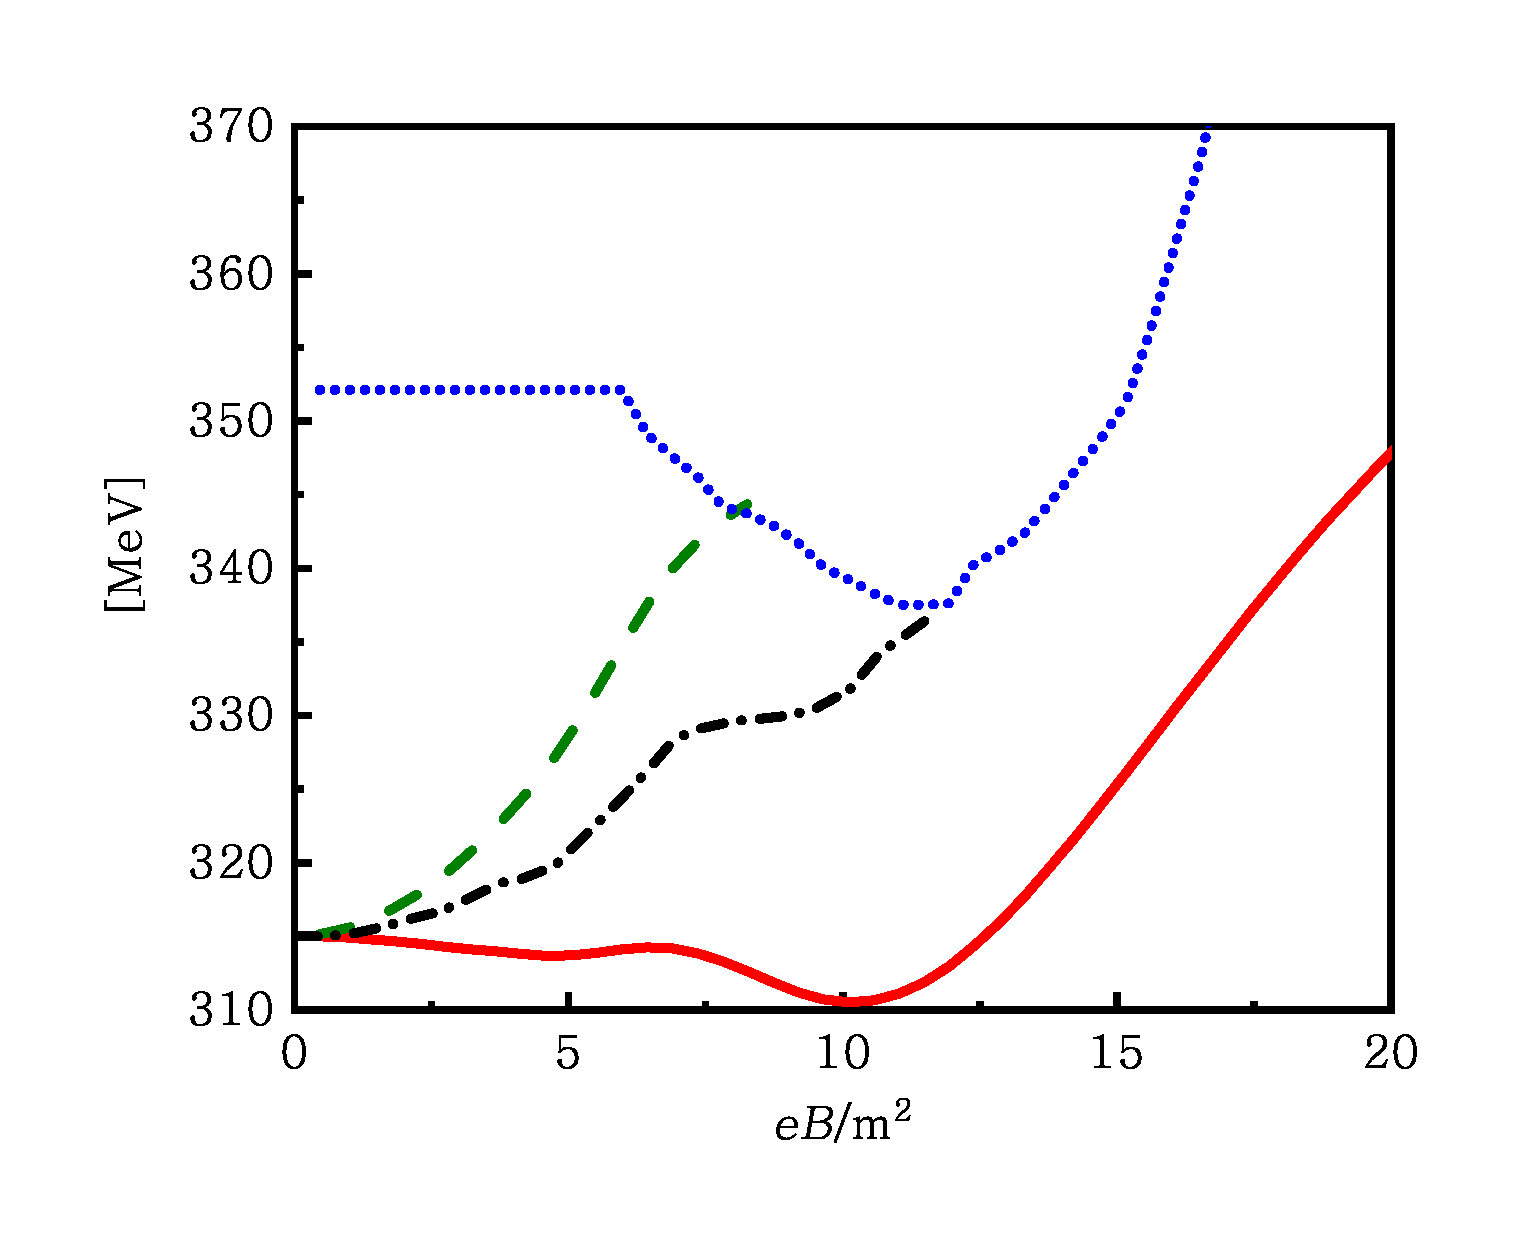
\includegraphics[width=0.6\textwidth]{3.eps}
    \label{fig:thirdpoint}
\end{figure}
With the model parameters mentioned in Sec.\ref{sec:2c},  $\mu_c^\text{I}$ (solid line) and $\mu_c^\text{II}$ (dashed line) for  $\text{BEC}_\text{I}$  and $\text{BEC}_\text{II}$  occurrences as  functions of the magnetic field have been given in Fig.\ref{fig:thirdpoint}.
%are denoted as $\mu_c^\text{I}$ (solid line) and $\mu_c^\text{II}$ (dashed line).
It is clearly shown the value of $\mu_c^\text{II}$   comes to be larger than that of $\mu_c^\text{I}$, with introducing magnetic field.
This explains that $\text{BEC}_\text{I}$ phase occurs firstly in the situation of finite magnetic field.
As $\text{BEC}_\text{I}$ has existed,  $\text{BEC}_\text{II}$ seems to occur sequentially.
Nevertheless, there exist no the pure  $\text{BEC}_\text{II}$ phase in the phase diagram.
The reason lies in the fact that not merely $\text{BEC}_\text{I}$ occur at relatively low $\mu$, but also $\text{BEC}_\text{II}$ (if exists) undergoes a crossover to the BCS phase at $eB \simeq 8 m_\pi^2$.
Indeed, for intermediate magnetic field, there is the position of the so-called BEC phase.
As depicted in Fig.\ref{fig:thirdpoint}, 
the BEC phase exists until
%the quark chemical potential decided by $\mu=M$ as dot line behaves as critical point for the BEC-BCS crossover.
%At $eB \simeq 8 m_\pi^2$,  $\text{BEC}_\text{II}$ phase disappears since the crossover to BCS phase has happened. In fact,
%there exist no possibility for  the imaginary $\text{BEC}_\text{II}$ phase with zero value of diquark condensate $s_B$, owing to   non-zero value of diquark condensate $s_B$ raises firstly.
%Therefore BEC phase with non-zero value of diquark condensates $s$ and $s_B$ appears in the phase diagram.
 the line of $\mu_c$ meets the line of $\mu_X$ at $eB \simeq 9 m_\pi^2$.
Obviously, it   corresponds to the threshold value of magnetic field $eB_{thr}$. This fact could explain the 
result for phase diagram Fig.\ref{fig:high}.



Moreover,  it is worthy being stressed that various of critical chemical potentials have the different $B$-dependence tendencies.
For $\text{BEC}_\text{II}$ occurrence, $\mu_c^\text{II}$  behaves as an increasing function of $eB$.
Also for BEC occurrence, the value of $\mu_c$ is  an almost  monotonic increasing function.
However, the value of $\mu_c^\text{I}$ is not a monotonic increasing function, but behaves as an evidently decreasing  function at $ 6 m_\pi^2 <eB < 10 m_\pi^2$ regime.
Keep in mind that $\mu_c^\text{I}$ can be understood as  the critical end point of chiral phase transition,
therefore the intermediate magnetic field makes   chiral phase transition occur at relatively low chemical potential.
It is totally different from the case  of magnetic catalysis, namely,  has  increasing tendency with magnetic field. Such a
phenomenon, inconsistency with magnetic catalysis,  may be regarded as inverse magnetic catalysis (IMC).
Owing to this IMC effect, the value of $\mu_c^\text{I}$ is always less than the value of BEC-BCS crossover. 
In this sense, the IMC happened in $T=0$ and intermediate value of magnetic field is responsible for the result in phase diagram.

To this end, one may wonder whether or not the IMC effect originates from the oscillation of three gaps.
For $\mu_X$, there exist oscillation behavior.
In our opinion, the oscillation behavior is main reason for the IMC effect for $\mu^\text{I}_c$.
In other words, the conclusion for IMC would not be invalid even though using more reasonable regulator function to remove non-physical oscillation. 
This point has been stressed in Ref.\cite{Duarte2015BEC}.

\subsection{Strong  field analysis for $\text{BEC}_\text{I}$ occurrence }
 When the magnitude of magnetic field is sufficiently large, the system dimension could be reduced to $1+1$ dimension. Then the summation in Eq.~\eqref{eq:criticalforq} has reduced to only one term
and the so-called lowest Landau Level (LLL) works.
After such a simplification, the first term  of R.H.S. in Eq.~\eqref{eq:criticalforq} may be rewritten as
\begin{equation}\label{eq:cond2}
 \frac{eB}{ 2\pi^2} \int h_{\Lambda,B}^{n=0}
\frac{ \sqrt{p_3^2 + M^2}}{p_3^2 + M^2 - \mu^2} dp_3.
\end{equation}
By using Eq.~\eqref{eq:cond2}, Eq.~\eqref{eq:criticalforq} can be simplified as
\begin{equation}\label{eq:cond3}
  \frac{1}{H'} = \frac{4}{\pi^2}\int h_\Lambda \frac{E}{E^2-\mu^2} p^2 dp + \frac{eB}{2\pi^2} \int h_\Lambda
  \frac{E}{E^2-\mu^2} dp,
\end{equation}
where the single-particle energy $E= \sqrt{p^2 +M^2}$.

Note that the magnetic field values considered in the following, $eB =14m_\pi^2$ and $eB =20 m_\pi^2$ (corresponding to approximately $0.25$ and $0.4$ $\text{GeV}^2$ respectively ) are referred to in the literature as strong magnetic fields.
One one hand, these values are representative of the fields expected in collision experiments, which are estimated to have magnitudes of the order $eB \sim 15 m_\pi^2$\cite{V2009ESTIMATE}.
On the other hand, 
it was found that at the magnetic field region $eB > \mu^2$, the destination between $\Delta$ and $\Delta_B$ gaps of the magnetized CFL phase becomes significant\cite{ferrer2005magnetic}.
The minimum value of  magnetic field region above can be estimated to $2\mu^2$ approximately.  
For our case,  in an intermediate chemical potential,
choosing such this magnetic field is reasonable.

On the one hand, for  our concerned $\text{BEC}_\text{I}$ occurrence, as shown in \ref{fig:thirdpoint}, the location of $\mu^{I}_c$ shift  to relatively larger chemical potential 
with given model parameter. As also depicted in Fig.\ref{fig:thirdpoint}, the value of $\mu_X$, determined by $\mu =M$,  is always larger than that of $\mu^{I}_c$.
Therefore the  $\text{BEC}_\text{I}$ phase exists still and the location of  $\text{BEC}_\text{I}$ becomes larger with 
increasing magnetic field.

On the other hand, once the axial anomaly is introduced,  the effective diquark coupling becomes $H' = H -\frac{1}{4}K'\chi$.
Therefore, the additional chiral-diquark interplay enhance the diquark coupling.
This is the essential reason that the axial anomaly raise the COE of chiral and diquark condensates and thus diquark BEC phase occur.


As shown  in Eq.~\eqref{eq:cond3}, effective diquark coupling is mainly determined by the value of the effective mass and chemical potential.
In order to show the magnetic effect, the chemical potential dependence in criterion equation are given at a specific value say, $\mu= 315$ MeV(zero-field).
As for the effective mass, at the given $\mu=315$MeV, our numerical results shows $M$ is an increasing function and $M \sim \sqrt{eB}$\cite{Gusynin1994Dimensional,Miransky2012Catalysis}.
In order to remove the magnetic effect from $M$, our discussions are organized by the following steps. As the first step, we assume that the effective   mass $M$ keeps unchanged with magnetic field. Then  we consider $B$ dependence of $M$ and turn to give a full analysis of the $H'$ behavior.
It is worthy being stressed that for our concerned $\text{BEC}_\text{I}$ occurrence, the effective mass only depends on the chiral-related parameter $G$ and $K$ and thus its variation with $B$ can be determined completely, even if the effective coupling $H'$ varies.

\begin{figure}[h]
  \caption{  The ratio of required effective coupling  for  the diquark $\text{BEC}_\text{I}$ phase transition, with chiral condensate (solid line) and without chiral condensate (dashed line). }
  \centering
    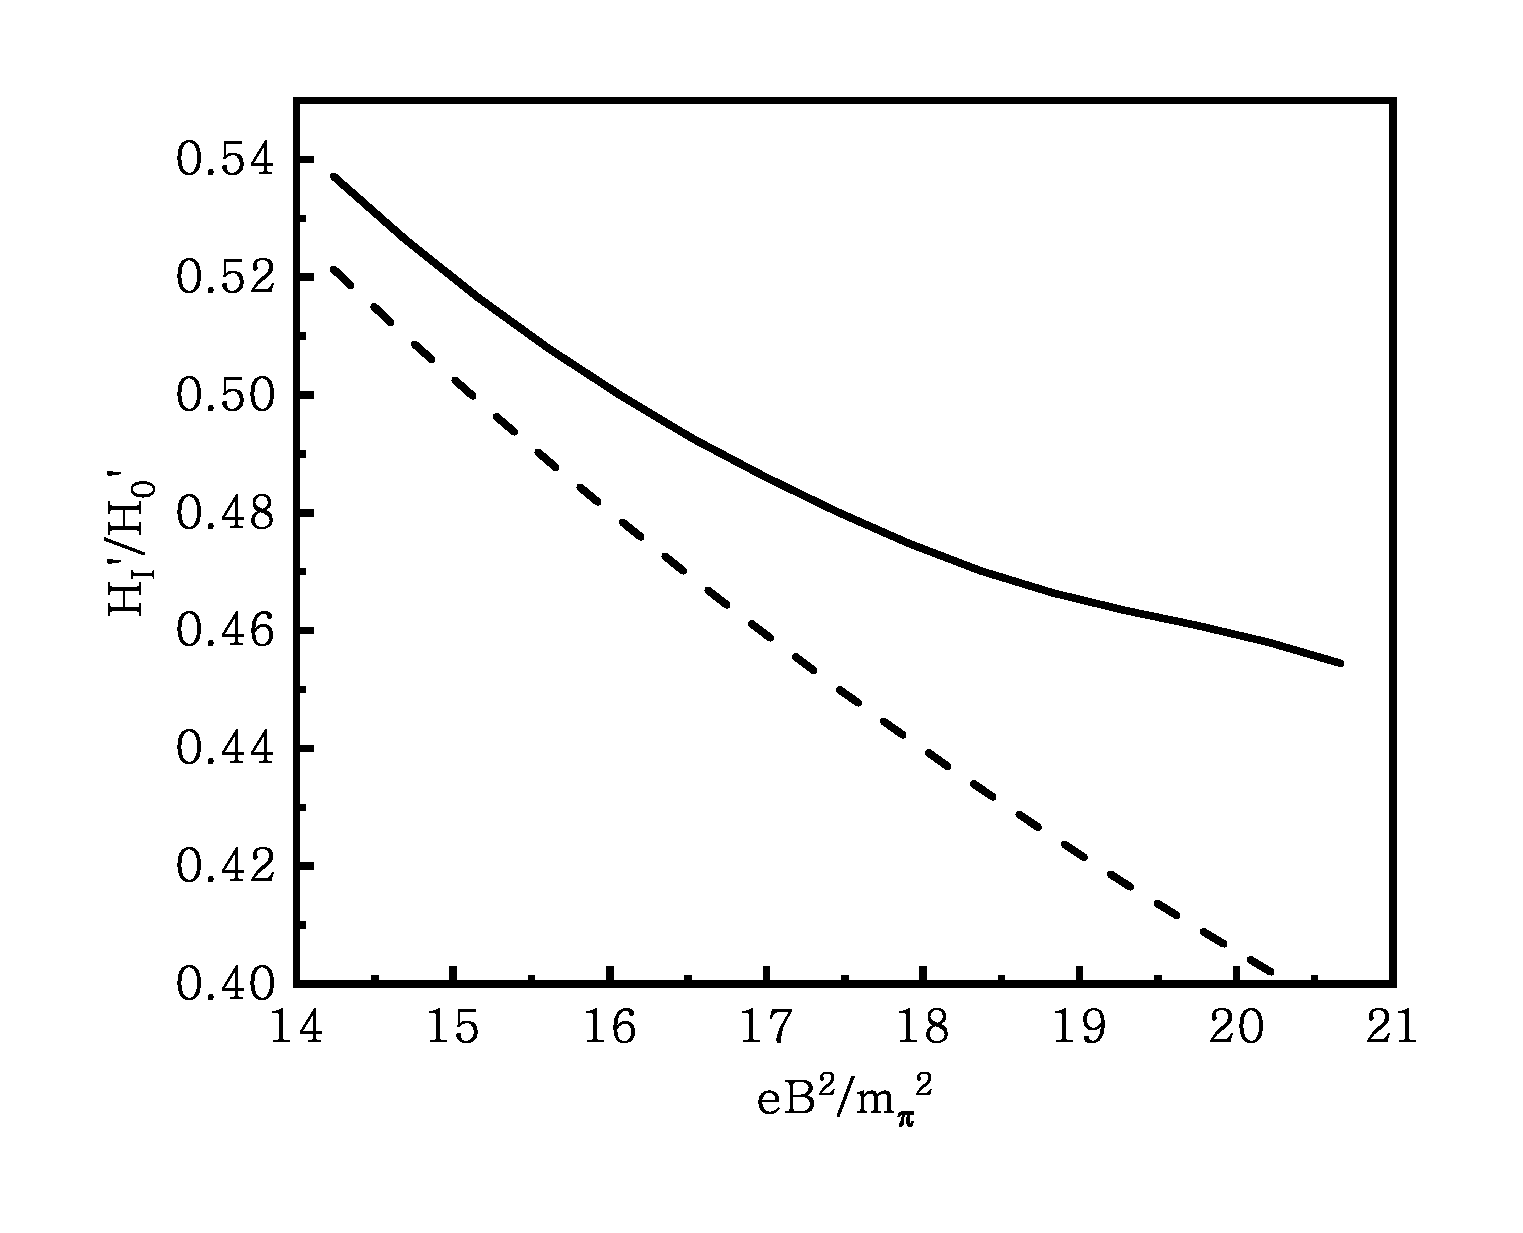
\includegraphics[width=0.5\textwidth]{high.eps}
    \label{fig:h}
\end{figure}





Incorporating the above dependence of $M$  into Eq.~\eqref{eq:cond3} through the  single particle energy $E$, we can give the magnetic field behavior of $H'$.
As depicted in Fig.\ref{fig:h}, the ratio of $H'_{I}/H'_0$ (dashed line)  displays a monotonic decreasing tendency, once the magnetic effect for chiral condensate is included. Here the diquark effective coupling $H'_0$  was obtained at zero-field limit. The decreasing tendency  indicates that strong field permits the occurrence of $\text{BEC}_\text{I}$.
%As the effective mass is assumed to be unchanged, it is easy to found that solid line is an obviously
%monotonic decreasing function of $B$ field. 
Note that, this is different from Fig.\ref{fig:thirdpoint}, where the value of $M$ is not constraint like this case.
The decreasing behavior as function of strong magnetic field indicates that strong field help  $\text{BEC}_\text{I}$ phase raise.

Once magnetic effect for chiral condensate is included, as shown by the dashed line, the effective coupling behavior manifest a monotonic decreasing function.
With increasing magnetic field, the $\text{BEC}_\text{I}$ phase not only remain valid, more importantly, its occurrence become possible even if the axial-anomaly induced interplay is suppressed relatively.
It implies that the strong field facilitates the $\text{BEC}_\text{I}$ occurrence originated by the chiral-diquark condensate interplay.


\begin{figure}[h]
\caption{  The ratio of  coupling $K'/K$ as  function of chemical potential at strong value of magnetic field.}
\centering
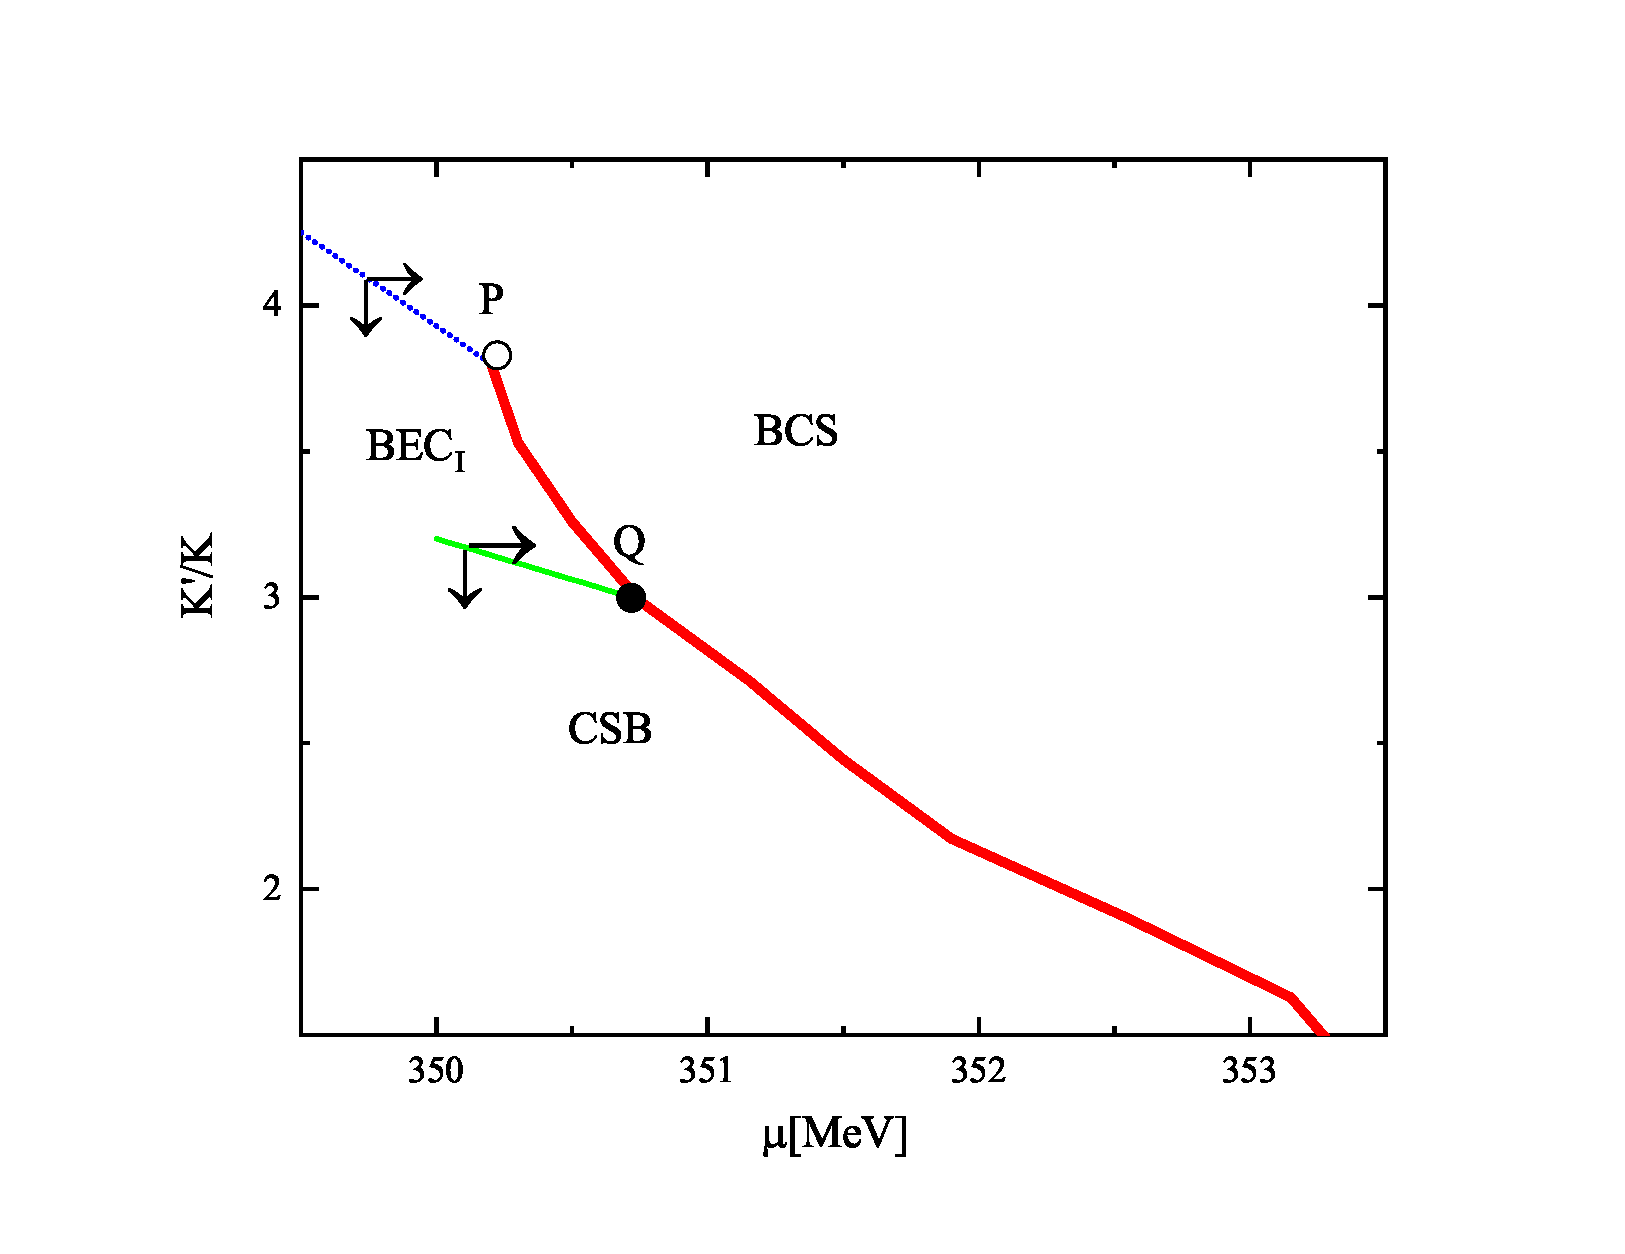
\includegraphics[width=0.6\textwidth]{kmu.eps}
\label{fig:kmu}
\end{figure}

Now let's turn to discuss the $B$-dependence for coupling $K'$ qualitatively.
We plot the phase diagram in the $\mu$-$K'$ plane at strong magnetic field in Fig.\ref{fig:kmu}
 One can recognize that for all choices of $K'$ there is  a first-order phase transition at some value of chemical potential.
  It is inevitable that existing $\text{BEC}_\text{I}$ as coexistence of chiral condensate $\chi$ and diquark condensate $s_B$ and BEC-BCS crossover.
 The line of $\text{BEC}_\text{I}$ and BEC-BCS crossover joint the line of first-order transition line at points $Q$ and P respectively.
 Point Q can be treated as the critical end point for chiral phase transition, since the parameter $\chi$
 is continuity.
 The distinction between $Q$ and $P$ is that point $P$ represents the transition between  $\text{BEC}_\text{I}$ and BEC-BCS crossover, not a critical end point.
 Then the chiral phase transition has returned to a first-order transition in point $Q$. 
If varying the magnetic field, the line of $\text{BEC}_\text{I}$ as well as  BEC-BCS crossover
shift to  relatively higher chemical potential in  a given value of $K'$.
If restricting to a given value of $\mu$ ,
as shown in Fig.\ref{fig:kmu}, the line of $\text{BEC}_\text{I}$ as well as  BEC-BCS crossover move to a lower value of $K'$.

%Within the NJL-type model, it is well known that  the coupling $H$
%represents the magnitude of diquark attractive interaction.
%Its appropriate value makes the BCS pairing and color superconducting %becomes possible.


%In order to explore the underlying mechanism of magnetic effects , we focus on
 %the effective coupling $H'$ and its magnetic dependence as diquark BEC phase occurs.
%Our discussion will be limited in the strong field regime, where an analytic treatment of magnetic
%effect becomes possible.  For the given diquark coupling $H$ as well as the chiral condensate related parameter
%$G$ and $K'$ , the behavior of $H'$  mainly represents the changes of the chiral-diquark interplay
%in the presence of strong magnetic field.
%Now let us  revisit these criterion equations for \cref{eq:criticalforq}.






%By removing the magnetic effect for chiral condensate,  the magnetic effect for diquark condensate can be clearly shown in the variation of effective coupling.
%For our purpose, firstly we ignore the magnetic dependence for the chiral condensate in order to simplify our problem.
%Then we include the magnetic field dependence in order to explain the realistic  condition.
%Here the value of chiral condensate is calculated at low chemical potential, being equivalent with the result
%obtained in Refs..



%In Fig.\ref{fig:h},  we plot the ratio of effective couplings $H'_\text{I}/H'_\text{0}$ and $H'_\text{II}/H'_\text{0}$   as functions of  magnetic field respectively in different given parameters.
%As shown in Fig.\ref{fig:h}.a, the effective coupling $H'_\text{I}$ is a monotonic decreasing function in a given value of chiral condensate.
%The decreasing behavior of $H'_\text{I}$ means that a strong field tends to facilitate the occurence of $\text{BEC}_\text{I}$  phase.
%In other words,   $\text{BEC}_\text{I}$ phase still remain valid, even though not  large value of the axial anomaly coupling $K'$  in the presence of strong magnetic background.
%%As shown in Fig.\ref{fig:h}, the effective coupling $H'_\text{I}$ is still a monotonic decreasing function, if ignoring the magnetic influence for chiral condensate.
%On the other hand, if the magnetic field dependence of the effective mass is included, it is observed as smaller value of the effective coupling and  a basically constant value of coupling.
%It means that the strong field case always bring out $\text{BEC}_\text{I}$  phase and critical point in the given parameters.
%
%
%As for  the  required effective diquark  coupling $H'_\text{II}$, it can be seen from Eq. that the effective coupling $H'_\text{II}$  keeps  unchanged, if magnetic dependence for the chiral condensate is  ignored.
%As depicted in Fig.\ref{fig:h}, once   the magnetic-dependence for the chiral condensate is taken into account, there exist a monotonic increasing tendency for coupling $H'_\text{II}$.
%Such result is very different from the case of effective coupling $H'_\text{I}$.
%It implies that  BEC  phase will disappear unless the axial anomaly induced interplay is enough strong.

%Or it means that, on the other hand, strong field the occurence.
%\begin{figure}[h]
%  \caption{  The ratio of required effective coupling $H'_\text{I}/H'_\text{0}$ as  functions of the magnetic field
%  at strong field regime. It is required at the chemical potential ($\mu=315MeV$ at zero field case). Blue solid line is given at the zero field case $M=470MeV$ and orange dashed line is for the value of  $M$ given at low chemical potential.}
%  \centering
%    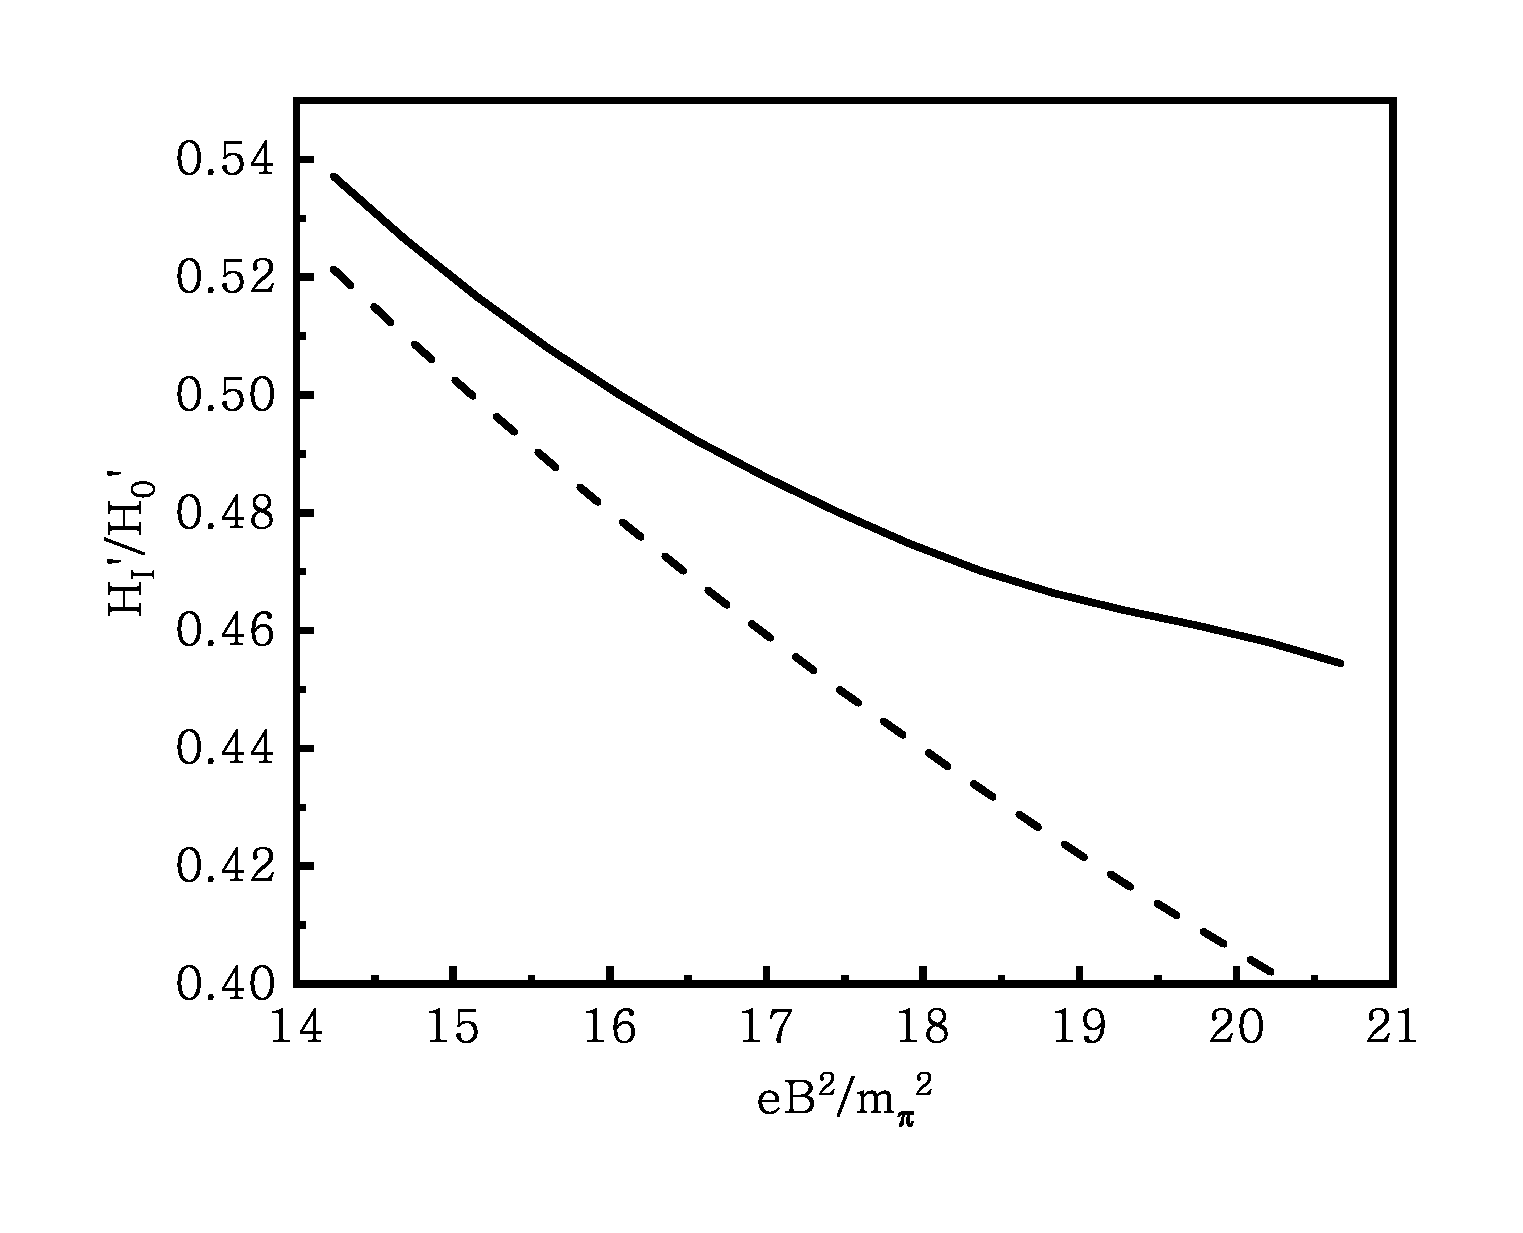
\includegraphics[width=0.5\textwidth]{high.eps}
%    \label{fig:high}
%\end{figure}



%
%\begin{figure}[h]
%  \caption{  The ratio of  coupling $K'/K_0$ as  functions of
%  chemical potential at different magnitude value of magnetic field.}
%  \centering
%    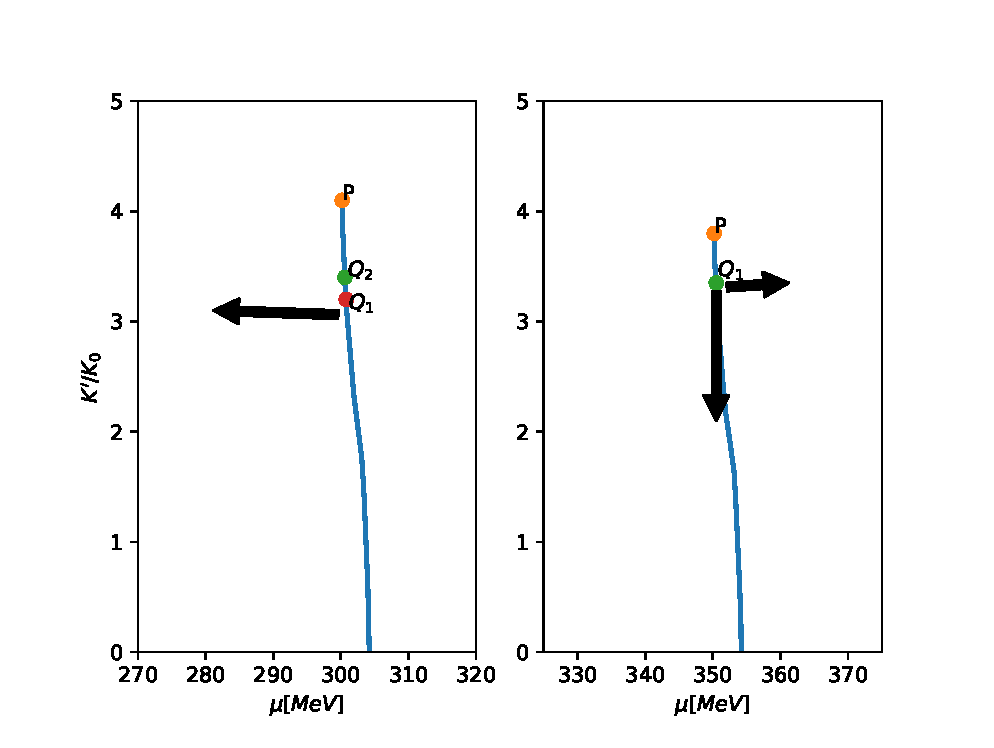
\includegraphics[width=0.6\textwidth]{muk.eps}
%    \label{fig:muk}
%\end{figure}
%
%%In fact, the discussion about the effective diquark coupling is under the varying of the coupling $K'$.
%At last,
%we plot the phase diagram in the $\mu$-$K'$ plane at different magnitude magnetic field in order to give a brief summary for our results.
%First we show the $\mu$-$K'$ phase diagram Fig.\ref{fig:muk} at a relatively not strong value of magnetic field. One can recognize that for all choices of $K'$ there is always a first-order phase transition at some value of chemical.
%And the value of chemical potential for the first-order phase transition increases with magnetic field.
%Such behavior can be treated as a magnetic catalysis.
%Same with the case of zero field, the line of BEC-BCS crossover meets the line of first-order transition line at $P$.
%It means that there exist BEC-BCS crossover and BEC phase under larger than the value of coupling $K'$ at point $P$.
%Compared with the case of zero field,  it was showed  the $\chi$SB phase and the CSC phase will be presented for smaller values of $K'$.
%Different with the zero field results obtained in Ref.,  the
%line of $\text{BEC}_\text{I}$ and BEC joint the line of first-order transition line at points $Q_1$ and $Q_2$ respectively.
%It was shown that  points $Q_2$ and  $P$ move down with magnetic field.
%Although it seems that the increasing behavior of chemical potential for first-order transition requires a larger value of coupling $K'$, the value of chemical potential for BEC-BCS crossover is an increasing function.
%Such behavior for BEC-BCS crossover  maintain that the point $P$ will not move up with magnetic field.
%On the other hand, the competition between  first-order transition and BEC-BCS crossover leads to this trend of change for point $P$ is not obvious.
%% This point can be also concluded by the fact that the effective required coupling increases with magnetic field at small value of magnetic field. The increasing value of coupling  $H'$ means that system requires larger value of coupling $K'$.
%
%In Fig.\ref{fig:muk}, the case of strong field was also depicted.
%It was shown that point $Q_2$ disappears from phase diagram.
%But  point $Q_1$ and $P$ located still at phase diagram .  It means that BEC phase has disappeared and there still exists a somewhat smaller value of coupling $K'$ to maintain the occurrence for $\text{BEC}_\text{I}$ phase and BEC-BCS crossover.


\section{Conclusion and discussions}

By incorporating the magnetized CFL matter into  a modified three-flavor NJL phenomenological model,
we have investigated the coexistence of chiral condensate and diquark condensate and the critical phenomena at $T=0$.
Based on the rotated electromagnetic mechanism in CFL matter, diquark condensate is split into two species, $s$ and $s_B$.
According to this fact, we have derived the NJL formalism of magnetized CFL matter with axial anomaly.


Different from the zero field results that the coexistence region  contains a diquark
BEC phase,  splitting of BEC phase was found at intermediate magnetic regime.
More precisely, $\text{BEC}_\text{I}$ phase (with $s_B \neq 0$, $s = 0$,
$\chi \neq 0$)
appears first,  the previous predicted BEC phase raises as follows.
For strong field regime, the original BEC vanishes and
$\text{BEC}_\text{I}$ phase occupies the COE phase completely.


As known that the BCS phase of magnetized CFL matter have been devoted sufficient researches.
Different from previous work, we focus on the critical phenomena happened in COE regime.
The splitting of BEC phase was observed and the specific $\text{BEC}_\text{I}$ phase was firstly proposed in our work.
The splitting of Bose Einstein Condensed phase represents the magnetic-field induced
violation of color-flavor symmetry.
The vanishing behavior for BEC phase indicates that magnetic field totally
destroys the critical phenomena in the COE regime.
%Within the model with axial anomaly, the nonzero magnetic background is stressed to play its key role on the coexistence and low-temperature critical phenomena.

Then we turn to investigate the underling mechanism by deriving the criterion condition for  $\text{BEC}_\text{I}$ and  $\text{BEC}_\text{II}$  occurrences.
 For the intermediate magnetic fields, say $eB < 10m_\pi^2$, the critical value of $\mu^{I}_c$ as functions of $eB$ has a decreasing tendency.
 It reflects that non-vanishing magnetic fields facilitate the Bose Einstein condensation of $s_B$, since the charged quarks becomes involved to $eB$ directly.

 Noticing that $\mu^{I}_c$ behaves as the critical end point of chiral transition, more importantly, the tendency can be understood as IMC, i.e.,
 the critical chemical potential for chiral phase transition shifts to a lower value with increasing magnetic field.
 In zero temperature QCD, the IMC phenomenon has already been pointed out in Ref.{}.
 There, the diquark BEC phase in two-color and two-flavor NJL model has some similar details with  $\text{BEC}_\text{I}$ discussed in the present work.
 In this sense, our result of IMC effect is not a strange phenomenon, and a general property in zero-temperature QCD physics.

 For strong magnetic field, say $eB > 11m_\pi^2$, the $\text{BEC}_\text{I}$ occurrence has some of significant features since analysis discussion is available.
  With the given model parameters, the $B$-dependence of $\mu_c^{I}$ is studied.
 As shown in Fig.\ref{fig:thirdpoint}, the location of $\text{BEC}_\text{I}$ is found to shift to larger quark chemical potential.
 %Therefore, strong field make it possible that the coexistence of $\chi$ and $s_B$ appears at a relatively high density.
 With the given chemical potential, on the other hand, the effective coupling $H'$ required for $\text{BEC}_\text{I}$
  is observed to become weaken for strong field.
% Because of Eq.~\eqref{eq:effectivecoupling}, it is clear that the strength of the relevant axial anomaly parameter $K'$ decreases with magnetic field.
 %Therefore, 
 As discussed in Sec., it is possible that strong fields makes it possible that the diquark-chiral coexistence appears when a relatively small axial anomaly coupling is chose.
It is known that the QCD with axial anomaly is usually suppressed at high densities.
In the situation with strong magnetic field, therefore, it is reasonable  a combination of  larger $\mu_c^I$ and  lower $K'$ corresponds to a more realistic physical environment.

In a realistic physical environment, e.g., magnetars, the influence of magnetic field
 can not be negligible.
If magnetars have color-superconducting cores, it is very likely that the present-discussed coexistence of $s_B$ and $\chi$ and the corresponding
critical phenomena provide key information for the observation of magnetars and understanding physics of magnetars.

A  further and detailed theoretical study of low-temperature QCD critical phenomena should incorporate the influences of quark bare masses, de-confinement term as well as finite temperature.
Under the compact star conditions, it is still unclear how to figure out these effects self-consistent at the same time.

\bibliographystyle{apsrev4-1}

\bibliography{bibfile}

\end{document}












